\documentclass[a4paper,article,oneside,11pt]{memoir}

% Cargamos todos los paquetes

\usepackage[utf8]{inputenc}
\usepackage[spanish,es-nodecimaldot,es-tabla]{babel}

\usepackage{fourier} % Cambiar la fuente a Utopia de Adobe
\usepackage{microtype} % Para mejorar un poco los algoritmos de justificación
\usepackage{graphicx}
\newsubfloat{figure} % Para poder incluir varias imágenes en una sola figura
% \usepackage{subcaption} % incluir varias imágenes en una sola figura con otra clase de documento

\usepackage{booktabs} % Crear tablas bonitas
\usepackage{hyperref} % Crear hipervínculos dentro del documentos
\usepackage{url} % Incluir enlaces a páginas web

\usepackage{float} % Para poner la H
\usepackage{rotating}
\usepackage{wasysym} % Incluir caritas felices 

\pagestyle{plain} % Cómo se van a ver encabezados y pies de página
% headings
% simple
% ruled
% Ruled
% companion

\title{Imágenes, tablas y un poco más}
\author{inm}

% Aquí termina el preámbulo y comienza el documento
\begin{document}

\maketitle

\noindent El objetivo del día de hoy es aprender a importar imágenes dentro del documento, a crear tablas y a usar \verb|\label| y \verb|\ref|. Como se habrán dado cuenta, usé \verb|\noindent| para iniciar el texto, esto es porque el primer párrafo de una sección suele escribirse sin sangría, mientras que los demás suelen escribirse con sangría, esto es útil cuando terminamos un párrafo con una ecuación o cuando un párrafo termina al final de la página, ya que así podremos distinguir el principio del siguiente párrafo.

Para comenzar un nuevo párrafo, basta dejar un espacio en blanco en el código, lo cual \LaTeX\ lo va a interpretar de forma correcta. Esta no es la única forma de comenzar un nuevo párrafo. También podemos usar el comando \verb|\par|. \par
En este caso no es necesario dejar la línea en blanco. Hay personas que usan \verb|\\| para comenzar párrafos o dejar más espacio éstos. Esto no es necesario y solamente les va a crear advertencias al momento de compilar un texto, evítenlo como la plaga. Si tal es la necesidad de dejar un mayor espacio entre los párrafos, se puede usar \verb|\setlength{\parskip}{\baselineskip}| o usar el paquete \texttt{parskip}.

Antes de importar nuestra primera imagen, tenemos que saber lo que es un \emph{float}, el cual es un contenedor que no puede ser ``roto''. Dos ejemplos de floats son \verb|figure| y \verb|table|, aunque el otro día vimos otro que es \verb|algorithm| e incluso podemos definir nuevos floats. Para incluir una imagen, podemos usar el comando \verb|\includegraphics|. 
\includegraphics[width=0.5\textwidth]{images/huuuu.png} Poner la imagen de esta forma no se ve muy bien, pues rompe la continuidad del texto. Para evitar esto usaremos \verb|figure|.

\begin{figure}[htp]
    \centering
    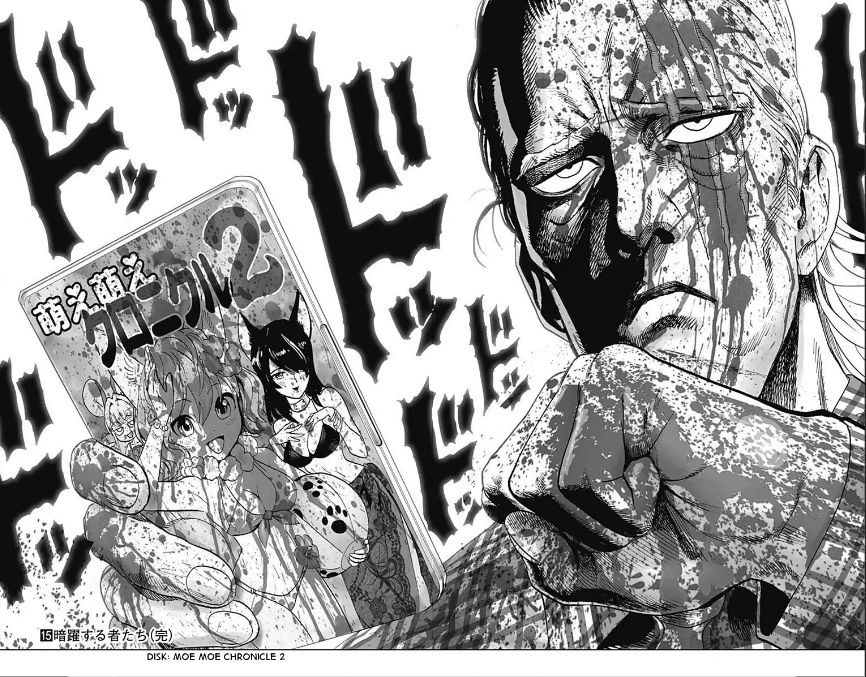
\includegraphics[width=0.8\textwidth]{images/king.png}
    \caption{El más fuerte del mundo.}
    \label{fig:king} 
\end{figure}

En la figura \ref{fig:king} nos encontramos por primera vez con el comando \verb|\label|, el cual nos permite ponerle un ``nombre'' por el cual nos podremos referir a una figura/tabla/ecuación/teorema dentro de \LaTeX\ por medio del comando \verb|\ref|. Para evitar confundirme, suelo ponerle \texttt{fig:nombre} a las figuras, \texttt{tab:nombre} a las tablas y de forma similar para otros labels.

Ahora veremos como incluir varias imágenes dentro de una sola figura. Dentro de \texttt{memoir} podemos usar el comando \verb|\subbottom|. Si estamos usando otra clase de documento, deberemos cargar un paquete de \texttt{subfig} o \texttt{subcaption}.

\begin{figure}[htp]
    \centering
    {
        \subbottom[Imagen 1]{
            
\includegraphics[width=0.45\textwidth]{images/ok.png}
        }
        \subbottom[Imagen 2]{
            
\includegraphics[width=0.45\textwidth]{images/suplex.png}
        }

        \subbottom[Imagen 3]{
            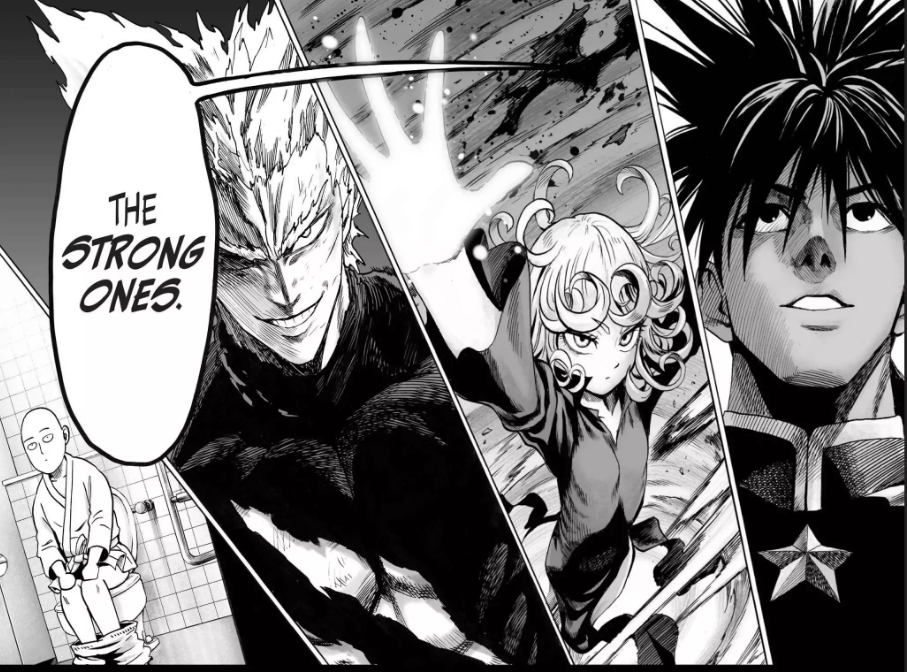
\includegraphics[width=0.45\textwidth]{images/juertes.png}
        }
    }
    \caption{Ejemplo de 3 imágenes en una figura con memoir.}
    \label{fig:3 figuras}
\end{figure}

% Comentado voy a poner cómo sería con subcaption
%\begin{figure}[htpb]
%    \centering
%    \begin{subfigure}[b]{0.45\textwidth}
%        
\includegraphics[width=\textwidth]{images/ok.png}
%        \caption{Imagen 1}
%    \end{subfigure} 
%    \hfill
%    \begin{subfigure}[b]{0.45\textwidth}
%        
\includegraphics[width=\textwidth]{images/suplex.png}
%        \caption{Imagen 2}
%    \end{subfigure}
%
%    \begin{subfigure}[b]{0.45\textwidth}
%        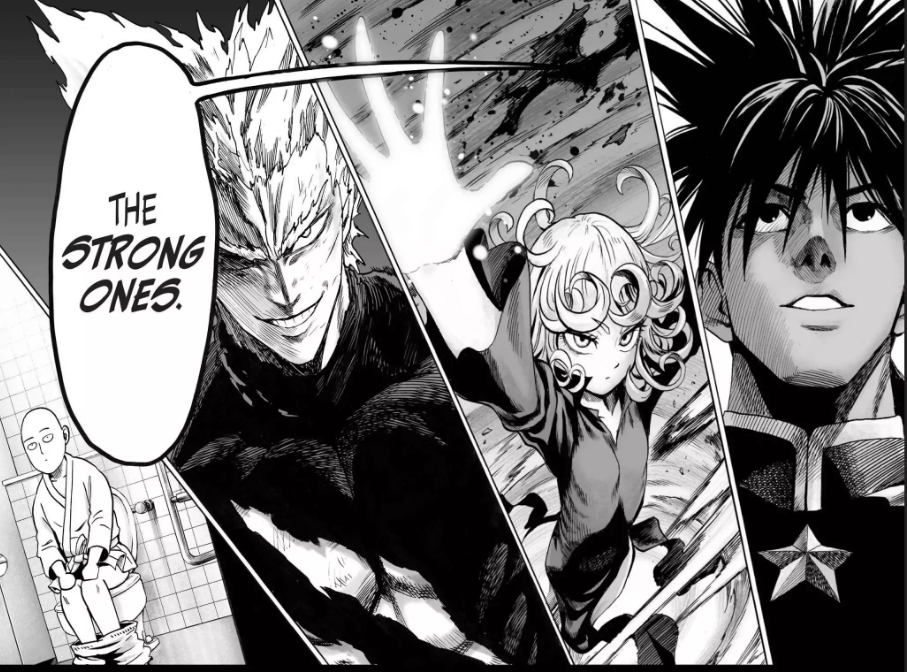
\includegraphics[width=\textwidth]{images/juertes.png}
%        \caption{Imagen 3}
%    \end{subfigure}
%    \caption{3 imágenes en una figura con \texttt{subcaption}}
%    \label{fig:varias 2}
%\end{figure}

Ahora crearemos tablas. Para esto, usaremos el ambiente \texttt{tabular}. Por ejemplo, 
\begin{tabular}{@{}ccc@{}}
    \toprule % la línea superior de la tabla
    soy & una & tablita \\ % \\ para ir a una nueva línea
    \midrule
    1 & 2 & 3 \\
    \bottomrule
\end{tabular}
es una tabla dentro del texto. Para evitar que esto suceda, debemos crear la tabla dentro de un float, con el ambiente \texttt{table}. Finalizaremos el día de hoy con varios ejemplos de tablas. Una pequeña guía: \url{https://inf.ethz.ch/personal/markusp/teaching/guides/guide-tables.pdf}.

\begin{table}[htp]
    \centering
    \begin{tabular}{@{}llr@{}}
        \toprule
        \multicolumn{2}{c}{Item} \\ 
        \cmidrule(r){1-2}
        Animal & Description & Price (\$)\\ 
        \midrule
        Gnat  & per gram  & 13.65 \\& each      & 0.01 \\
        Gnu   & stuffed   & 92.50 \\Emu   & stuffed   & 33.33 \\
        Armadillo & frozen & 8.99 \\ 
        \bottomrule
    \end{tabular}
    \caption{Tablita más elegante}
    \label{tab:tablita animales}
\end{table}

\begin{table}[htp]
    \centering
    \begin{tabular}{@{}lrrrr@{}}
        \toprule
        & \multicolumn{2}{c}{A} & \multicolumn{2}{c}{B} \\
        \cmidrule(lr){2-3} \cmidrule(l){4-5}
        & Weight (lbs.) & Weight (lbs.) & Price & Price \\
        \midrule
        Mileage (mpg) & $-108.4^{***}$ & $-91.22^{***}$ & $-49.51$ & $21.85$ \\
         & $(-11.60)$ & $(-10.34)$ & $(-0.57)$ & $(0.29)$ \\[0.5em]
        Car type & & $-550.1^{***}$ & & $3673.1^{***}$ \\
        & & $(-4.96)$ & & $(5.37)$ \\[0.5em]
        Weight (lbs.) & & & $1.747^{***}$ & $3.465^{***}$ \\
        & & & $(2.72)$ & $(5.49)$ \\[0.5em]
        Constant & $5328.8^{***}$ & $5125.7^{***}$ & $1946.1^{***}$ & $-5853.7^{***}$ \\
        & $(25.85)$ & $(27.93)$ & $(0.54)$ & $(-1.73)$ \\
        \midrule
        Observations & $74$ & $74$ & $74$ & $74$ \\
        \bottomrule
    \end{tabular}

    \smallskip
    {\raggedright\scriptsize \hspace{3.5em}$t$ statistics in parentheses \hfill \\
    \hspace{3.5em}$^* \; p < 0.05$,\quad $^{**} \; p < 0.01$,\quad $^{***} \; p < 0.001$\hfill}
    \caption{Ejemplo de tabla de economistas \smiley}
    \label{tab:tablita eco}
\end{table}

\begin{sidewaystable}
    \begin{center}
        \centering
        \begin{tabular}{@{}lcccccccc@{}}
            \toprule
            & \multicolumn{8}{c}{Estados} \\
            \cmidrule(lr){2-9}
            Simulación & 0 & 1 & 2 & 3 & 4 & 5 & 6 & 7\\
            \midrule
            1 & 0.00034 & 0.0145299 & 0.1274387 & 0.3560564 & 0.3583864 & 0.1285187 & 0.0144499 & 0.00028\\
            2 & 0.00028 & 0.0146999 & 0.1282787 & 0.3590564 & 0.3536865 & 0.1286687 & 0.0149899 & 0.00034\\
            3 & 0.00026 & 0.0132299 & 0.1277687 & 0.3570464 & 0.3593864 & 0.1287287 & 0.0132499 & 0.00033\\
            4 & 0.00028 & 0.0137499 & 0.1305487 & 0.3564864 & 0.3562664 & 0.1280987 & 0.0142099 & 0.00036\\
            5 & 0.00029 & 0.0151398 & 0.1281787 & 0.3577464 & 0.3581064 & 0.1269787 & 0.0132399 & 0.00032\\
            \addlinespace
            6 & 0.00029 & 0.0134299 & 0.1283587 & 0.3584264 & 0.3567164 & 0.1281687 & 0.0142799 & 0.00033\\
            7 & 0.00023 & 0.0144499 & 0.1281587 & 0.3537265 & 0.3581864 & 0.1304587 & 0.0144499 & 0.00034\\
            8 & 0.00029 & 0.0138399 & 0.1273387 & 0.3570664 & 0.3566264 & 0.1294387 & 0.0150198 & 0.00038\\
            9 & 0.00033 & 0.0148499 & 0.1283287 & 0.3543365 & 0.3592664 & 0.1285487 & 0.0141099 & 0.00023\\
            10 & 0.00036 & 0.0145499 & 0.1284987 & 0.3562664 & 0.3574764 & 0.1283787 & 0.0141999 & 0.00027\\
            \bottomrule
        \end{tabular}

        \caption{Ejemplo de tabla en horizontal.}
        \label{tab:tablita ancha}
    \end{center}
\end{sidewaystable}

\end{document}